%-----------------------
% Title page
%-----------------------
\begin{titlepage}
    \centering

    \textsc{ELEC4630 Assignment 3}\\
    \vspace{9cm}

    \rule{\linewidth}{0.5pt}\\

    \vspace{1em}
    \LARGE\textsc{Question 1}\\
    \vspace{1em}

    \LARGE\uppercase{\textbf{{Personal GitHub Blog}}}\\

    \rule{\linewidth}{2pt}\\

    \vfill

    \normalsize{Deren Teo (45285545)}
    \vspace{1cm}

  \end{titlepage}

%-----------------------
% Document body (this one's not a report)
%-----------------------
\section*{Summary}

This question required the creation of a personal blog on GitHub using the \texttt{fast\_template} provided by fastai. The blog is available at: https://deren-teo.github.io/.

The following pages provide an number of screenshots as evidence of the work.

\subsection*{Sample from ``How to start a blog post'' (14 May, 2023)}

\begin{figure}[!ht]
    \centering
    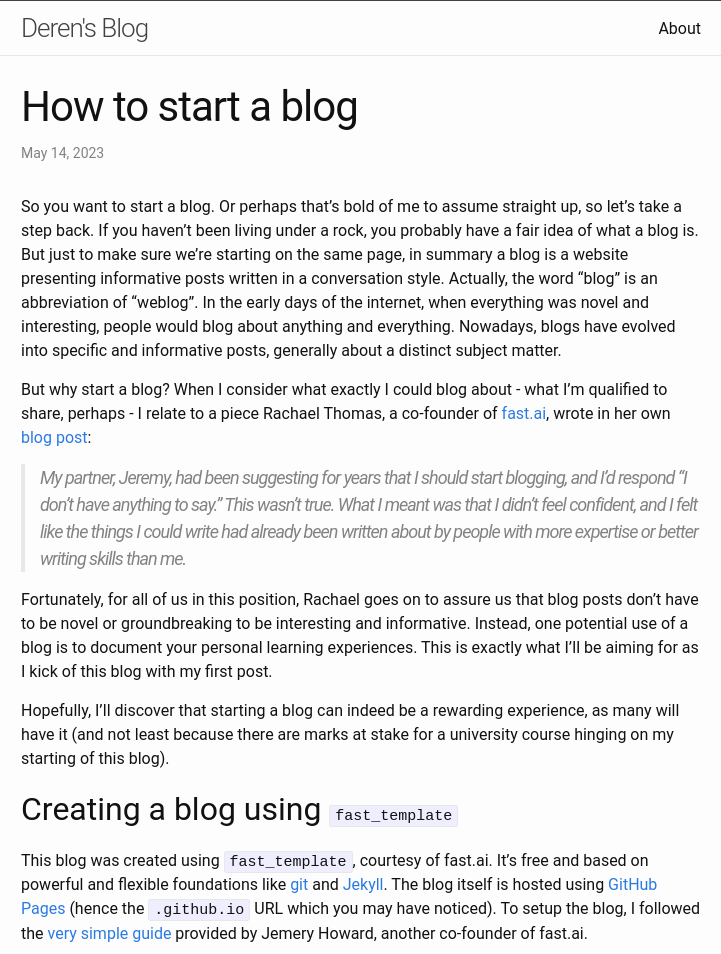
\includegraphics[width=0.9\textwidth]{images/q1_sample_of_post_1.png}
\end{figure}

\newpage

\subsection*{Sample from ``PyTorch on Windows with GPU'' (17 May, 2023)}

\begin{figure}[!ht]
    \centering
    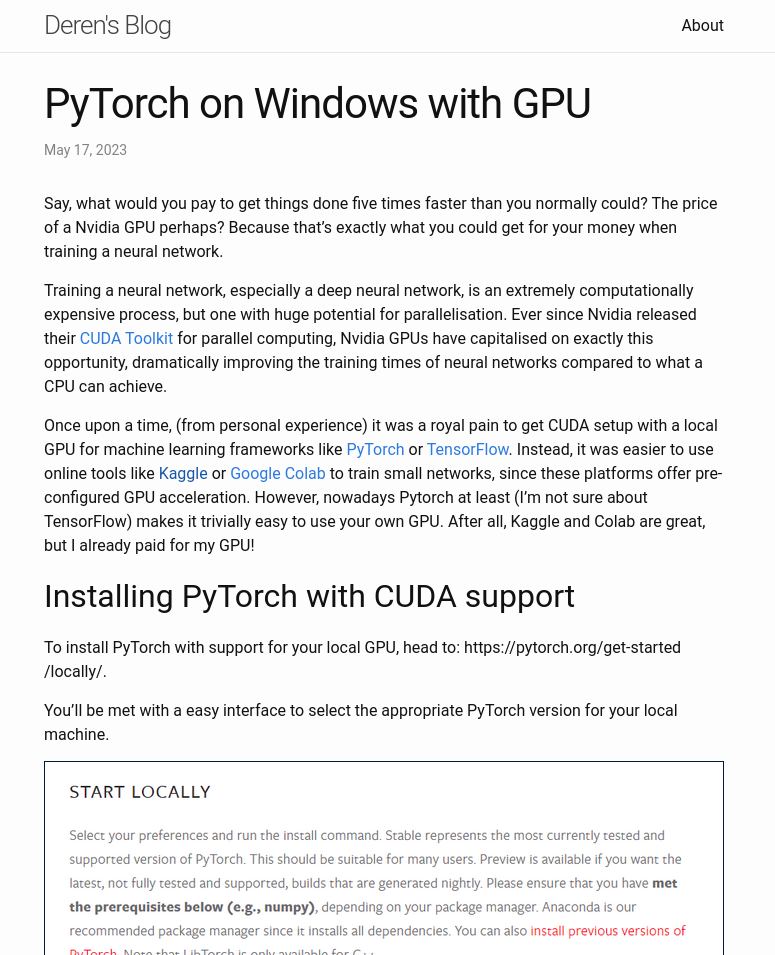
\includegraphics[width=\textwidth]{images/q1_sample_of_post_2.png}
\end{figure}

\newpage

\subsection*{Sample from ``Image classification using pre-trained networks'' (20 May, 2023)}

\begin{figure}[!ht]
    \centering
    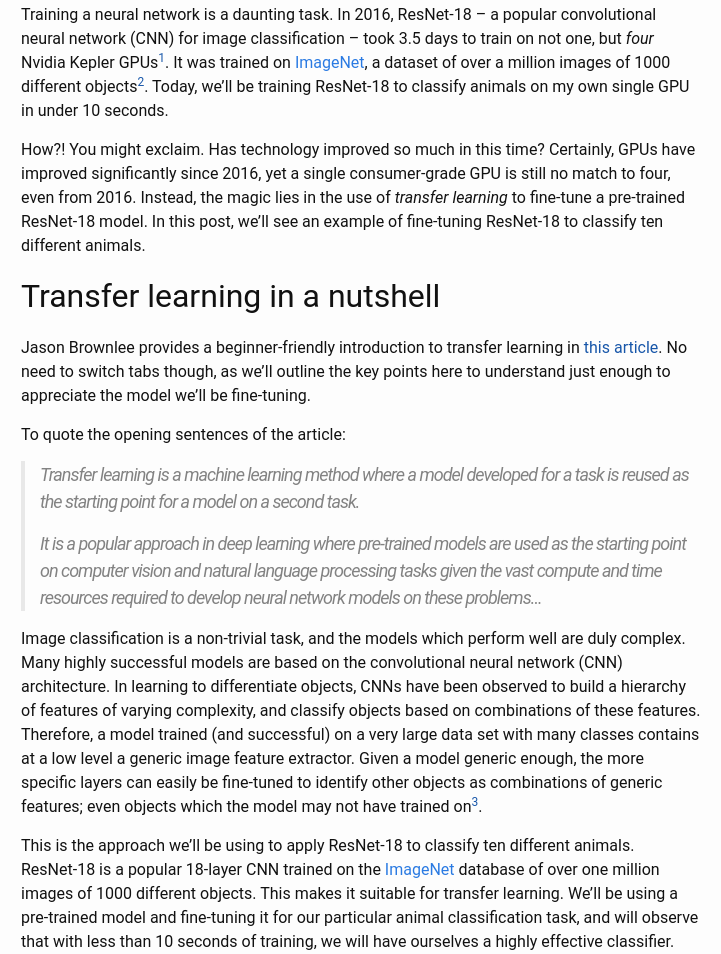
\includegraphics[width=\textwidth]{images/q1_sample_of_post_3.png}
\end{figure}

\newpage

\subsection*{Sample from ``Visualising ResNets using t-SNE'' (25 May, 2023)}

\begin{figure}[!ht]
    \centering
    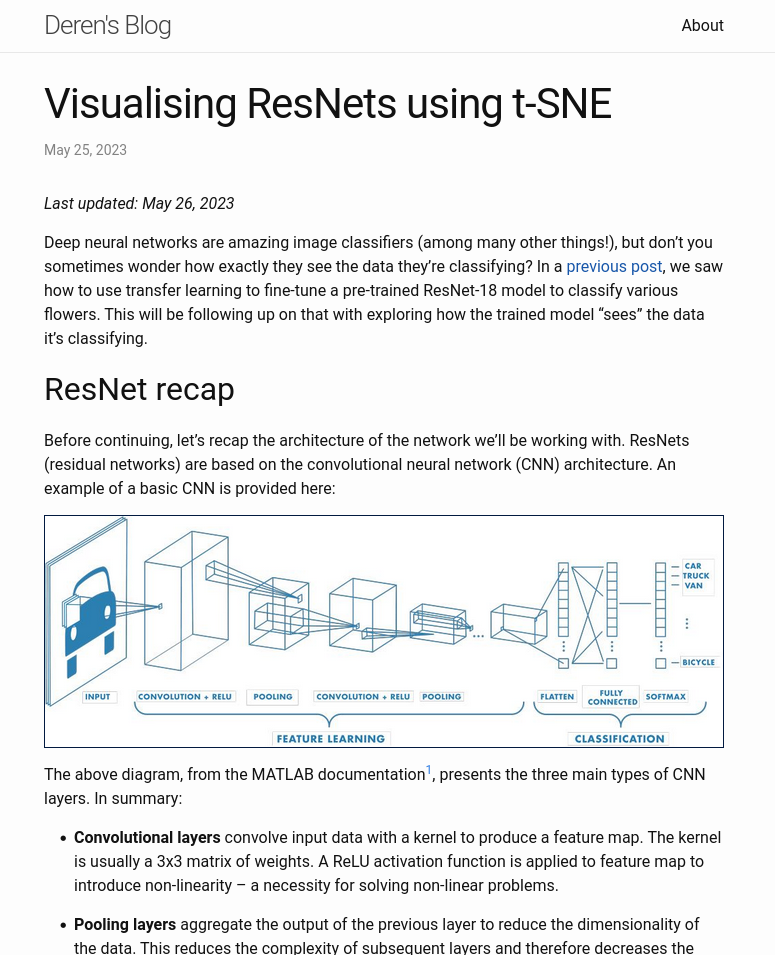
\includegraphics[width=\textwidth]{images/q1_sample_of_post_4.png}
\end{figure}
